% !TEX root = main.tex

\section{IO管理与磁盘调度}
控制设备和内存或CPU之间的数据传送方式:
\begin{itemize}
    \item 程序控制(programmed IO):需要不断读取IO控制器的状态寄存器,才能决定是否读写数据
    \item 中断驱动方式(interrupt-driven IO):IO设备主动打断CPU运行并请求服务
    \item 直接内存访问(Direct Memory Access, DMA):直接在IO设备和内存之间开辟直接的数据交换通路
\end{itemize}

假脱机技术(Simultaneous Peripheral Operations On Line, SPOOL)/虚拟设备技术:
专门利用一道程序来完成对设备的IO操作,而无需使用外围IO处理机
\begin{figure}[H]
    \centering
    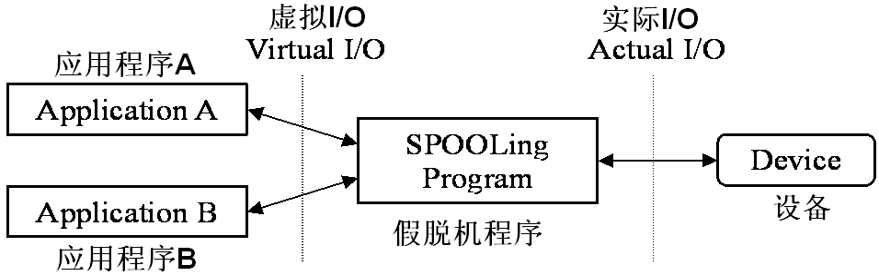
\includegraphics[width=0.7\linewidth]{fig/SPOOLing.png}
\end{figure}
优点是高速虚拟IO操作,实现对独享设备的共享

IO缓冲:CPU快IO慢,提高外设利用率,尽可能使外设处于忙的状态(多道程序并发);增加缓冲区有利于提高命中率,操作系统采用软件方法实现缓冲技术
\begin{itemize}
    \item 单方向缓冲:单缓冲、双缓冲、环形缓冲
    \item 双方向缓冲:缓冲池(buffer pool)
    \item 循环缓冲
\end{itemize}

磁盘调度算法
\begin{itemize}
    \item 先来先服务FCFS:公平简单,平均寻道距离大
    \item 最短寻找时间优先(shortest seek time first, SSTF):与当前磁头邻近的磁道,性能比FCFS好,可能出现饥饿;移臂距离最小
    \item 电梯算法/扫描算法SCAN:比较实用的调度算法:在最短寻找时间优先算法的基础上规定了磁头的方向,不利于磁头一端的访问请求
    \item 循环扫描算法C-SCAN:到头会回到另一侧重新开始,移臂方向改变最少
\end{itemize}

Windows支持两类RAID配置
\begin{itemize}
\item 硬件RAID:若干独立的物理磁盘,通过磁盘控制器或磁盘存储柜,组合成逻辑磁盘。冗余信息的创建和重新生成由控制器负责处理
\item 软件RAID:不连续的磁盘空间通过容错软件磁盘驱动程序(Fault-Tolerant software DISK driver, FTDISK)组合成逻辑分区。Windows的软件RAID机制实现了RAID1(镜像)和RAID5(交错块分布式奇偶校验)
\end{itemize}